\chapter{Developer Biography}\label{chap:biography}

\begin{center}
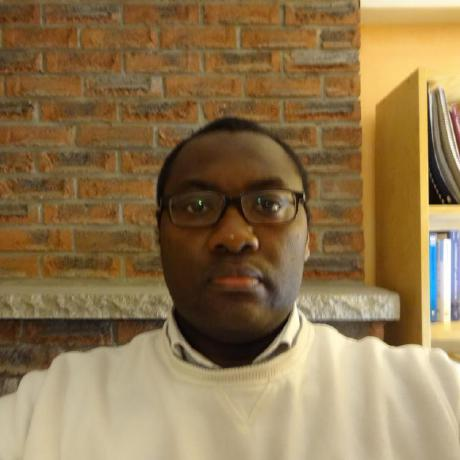
\includegraphics[scale=0.32]{../../francais/images/XavierNOUNDOU-2}
\captionof{figure}{Portrait of Xavier.}
\label{fig:xaviernoumbis}
\end{center}

\textbf{\myfullacademicname} is a Cameroonian
born on September~$16$ $1983$ in DOUALA (LITTORAL region, CAMEROON).

Xavier is a ''Diplom--Informatiker (\diplinf)'' of
the \textbf{University of Bremen, Bremen, Bremen, GERMANY} (May~$25$, $2007$).

\begin{comment}
Pendant ses \'etudes de \diplinf,
Xavier a travaill\'e pendant $25$~mois comme
d\'eveloppeur--logiciel (temps--partiel) \`a
\company{\bergmann} dans la ville de Rellingen
(Hambourg, Allemagne).

Juste apr\`es l'obtention de son \diplinf,
Xavier a travaill\'e $21$~mois comme d\'eveloppeur--logiciel--junior
\`a \company{\siemens} dans la ville d'Erlangen
(Bavi\`ere, Allemagne).

Xavier a quitt\'e ''\siemens'' en $2009$ pour poursuivre
des \'etudes doctorales Ph.D. en analyse statique des programmes
informatiques au laboratoire de recherche \company{Watform}
de \company{l'universit\'e de Waterloo}.

En $2012$, Xavier a travaill\'e $8$ mois en tant
que ''stagiaire doctorant Ph.D.'' dans l'\'equipe
de compilation \emph{Java Just--In--Time Compiler (J~$9$)}
de \company{IBM Toronto Software Lab} \`a Markham (Ontario, Canada).

Xavier quitte le labratoire de recherche ''Watform''
en Mars~$2015$.

Xavier lit, \'ecrit, et parle courament le Fran\c{c}ais,
l'Anglais, et l'Allemand.
\end{comment}